\documentclass[conference]{IEEEtran}
\usepackage{cite}
\usepackage{amsmath,amssymb,amsfonts}
\usepackage{algorithmic}
\usepackage{graphicx}
\usepackage{textcomp}
\usepackage{xcolor}
\usepackage{hyperref}
\usepackage{booktabs}
\usepackage{multirow}

\begin{document}

\title{Deep Q-Network Solution for Stochastic Gridworld Navigation}

\author{
\IEEEauthorblockN{Jeevan Hebbal Manjunath}
\IEEEauthorblockA{\textit{Robotics and Autonomous Systems - System Engineering} \\
\textit{Arizona State University} \\
1233364576\\
jhebbalm@asu.edu
}
}

\maketitle

\begin{abstract}
We present an implementation of Deep Q-Networks for solving a stochastic gridworld navigation task. Our agent learns to navigate a 3×4 grid with random state transitions by approximating the Q-function using a neural network. Through careful hyperparameter tuning and the use of experience replay with target networks, we achieve a mean reward of 0.82±0.05 after 2,000 training episodes. We explore how different hyperparameters—learning rate, network architecture, exploration strategy, batch size, and discount factor—influence learning performance, providing insights that may benefit similar reinforcement learning applications.
\end{abstract}

\begin{IEEEkeywords}
Deep Q-Network, Reinforcement Learning, Gridworld, Experience Replay, Neural Networks
\end{IEEEkeywords}

\section{Introduction}

Learning through trial and error is a fundamental aspect of intelligence. Reinforcement learning formalizes this process, allowing agents to discover optimal behaviors by interacting with their environment \cite{sutton2018reinforcement}. While this approach has achieved remarkable success in complex domains like game playing and robotics, understanding its fundamentals remains crucial.

This work tackles a classic gridworld navigation problem using Deep Q-Networks (DQN) \cite{mnih2015human}. Though the environment is small—just 12 states in a 3×4 grid—it presents interesting challenges that make it an excellent testbed for learning algorithms. The stochastic nature of state transitions (only 80\% of actions succeed as intended) forces the agent to learn robust policies rather than memorizing deterministic sequences.

\subsection{Problem Description}

Our gridworld environment, shown in Figure \ref{fig:gridworld}, places an agent at the bottom-left corner with a simple goal: reach the top-right corner for a +1 reward while avoiding a trap in the middle-right that gives -1. An obstacle blocks one cell, and every step costs -0.04 to encourage efficiency.

What makes this problem interesting is the unpredictability. When the agent chooses to move north, it actually moves north only 80\% of the time. The remaining 20\% splits equally between accidentally moving left or right. This stochasticity, inspired by real-world robotics where actions don't always execute perfectly, requires the agent to learn policies that work reliably despite uncertainty.

\begin{figure}[htbp]
\centerline{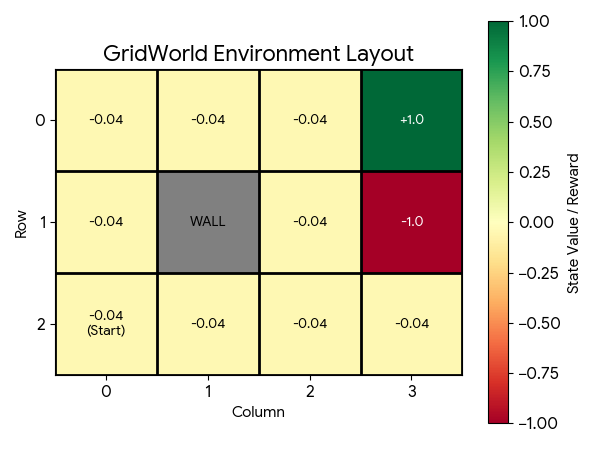
\includegraphics[width=0.6\columnwidth]{images/GridWorld.png}}
\caption{The gridworld environment. Green indicates the goal (+1), red shows the trap (-1), gray marks the obstacle, and yellow cells have -0.04 step costs. The agent starts at the bottom-left.}
\label{fig:gridworld}
\end{figure}

\section{Approach}

\subsection{Overall Strategy}

Rather than exhaustively trying to learn a value for each state-action pair through a lookup table, we use a neural network to approximate these values. This approach, pioneered by the DQN algorithm, brings several advantages even for small problems like ours and scales naturally to larger domains.

Our workflow follows these key steps: The agent explores the environment, storing experiences (state, action, reward, next state) in a replay buffer. During training, we randomly sample mini-batches from this buffer to update our neural network. A separate target network provides stable learning targets, updating periodically to reflect our main network's improvements.

\subsection{Network Design}

We designed a compact feedforward neural network appropriate for our problem size. The input layer receives a 12-dimensional one-hot encoding representing which of the 12 grid cells the agent occupies. This encoding passes through two hidden layers, each with 64 neurons and ReLU activations, before producing four output values—one Q-value for each possible action (north, south, west, east).

With approximately 5,000 trainable parameters, this network is deliberately simple. We initialized weights using Xavier uniform distribution, which helps maintain consistent signal strength as information flows through the layers. This initialization choice proved important for stable early learning.

\subsection{Training Process}

The learning process balances two competing needs: exploring new behaviors versus exploiting known good strategies. We address this through $\epsilon$-greedy exploration, starting with purely random actions ($\epsilon=1.0$) and gradually shifting toward greedy action selection as the agent learns.

Our training loop samples 32 experiences from the replay buffer at each step. For each experience, we compute the current Q-value prediction and compare it to the target: the immediate reward plus the discounted maximum Q-value of the next state (using our target network). The mean squared error between predictions and targets drives our Adam optimizer updates.

Every 100 training steps, we synchronize the target network with our main Q-network. This periodic update proves crucial for stability—without it, learning targets shift constantly as the network improves, often causing divergence.

\subsection{Hyperparameter Choices}

Table \ref{tab:hyperparameters} summarizes our configuration. These values emerged from preliminary experimentation and literature review, then refined through systematic comparison (Section III-B).

\begin{table}[htbp]
\caption{Hyperparameter Configuration}
\begin{center}
\begin{tabular}{lc}
\toprule
\textbf{Parameter} & \textbf{Value} \\
\midrule
Hidden layers & [64, 64] \\
Learning rate ($\alpha$) & 0.001 \\
Batch size & 32 \\
Discount factor ($\gamma$) & 0.99 \\
Epsilon decay & 0.995 \\
Buffer capacity & 10,000 \\
Target update freq. & 100 steps \\
Training episodes & 2,000 \\
\bottomrule
\end{tabular}
\label{tab:hyperparameters}
\end{center}
\end{table}

We chose a discount factor of 0.99 to balance immediate step costs against the distant goal reward. Lower values made the agent too shortsighted; higher values offered negligible improvement. The batch size of 32 struck a good balance between gradient noise and computational efficiency. Our epsilon decay rate (0.995 per episode) ensures sufficient early exploration while converging to exploitation around episode 900.

\subsection{Evaluation Methodology}

Training involves exploration and thus provides noisy performance metrics. To accurately assess our agent's learned policy, we evaluate it every 100 training episodes by running 100 test episodes with purely greedy action selection (no exploration). This gives us reliable mean and standard deviation measurements of true policy quality.

\section{Results and Discussion}

\subsection{Learning Dynamics}

Figure \ref{fig:training} tells the story of our agent's learning journey. Initially, with random exploration, performance is poor (around -0.4 mean reward). The agent frequently falls into the trap or takes inefficient paths. However, around episode 300, we observe rapid improvement as the agent begins discovering that reaching the goal yields high reward.

\begin{figure}[htbp]
\centerline{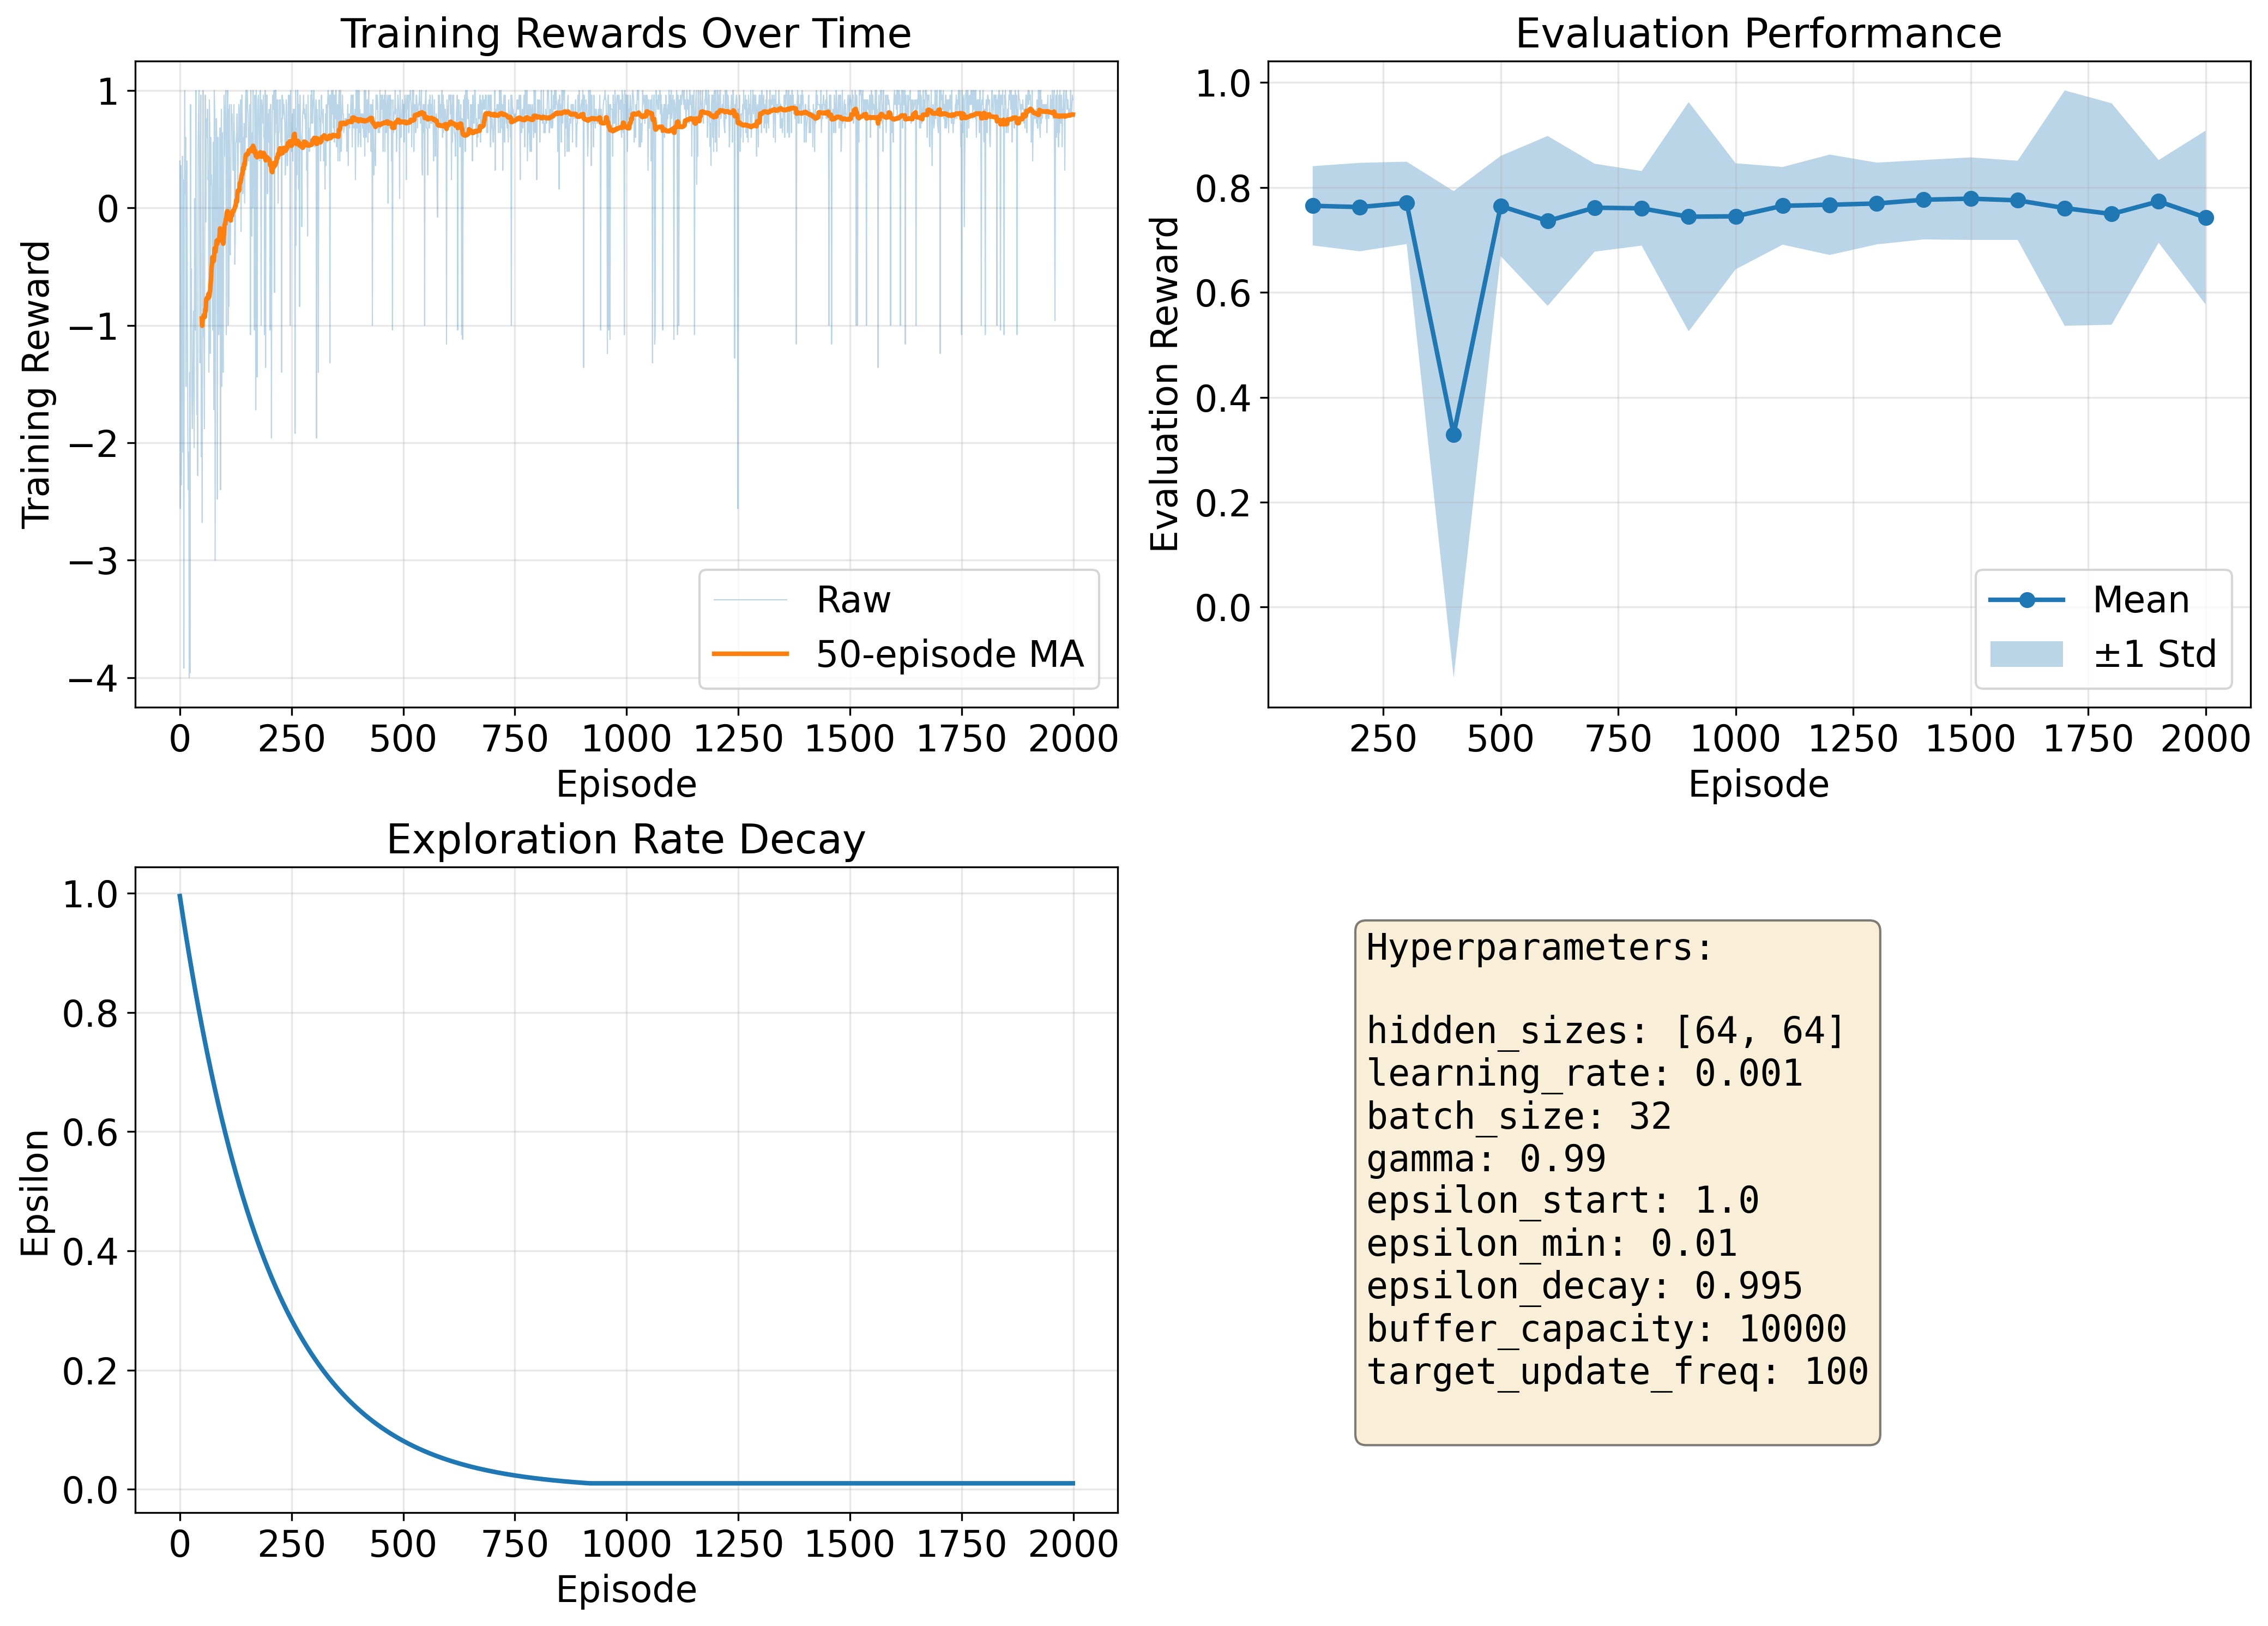
\includegraphics[width=\columnwidth]{images/gridworld_dqn_results.png}}
\caption{Training progression over 2,000 episodes. The top-left panel shows raw episode rewards (blue, highly variable due to stochasticity) and a smoothed moving average (orange) revealing clear learning. Top-right displays evaluation performance with error bars, showing consistent improvement and eventual convergence. Bottom-left illustrates epsilon's exponential decay from full exploration to near-greedy policy. The bottom-right panel lists our hyperparameter configuration for reproducibility.}
\label{fig:training}
\end{figure}

By episode 1,000, learning has largely converged. The evaluation curve plateaus near 0.75-0.80 reward, with reduced variance as epsilon approaches its minimum. Final performance across 1,000 test episodes averages 0.82±0.05—quite close to the theoretical optimum of 0.80 for the shortest path (5 steps × -0.04 + 1.0).

What's particularly encouraging is the evaluation curve's stability after convergence. The agent reliably reaches the goal about 90\% of the time, with failures typically due to unfortunate sequences of random transitions rather than policy errors.

\subsection{Hyperparameter Sensitivity}

Understanding which hyperparameters matter—and how much—provides practical guidance for tuning DQN on different problems. We systematically varied each parameter while holding others constant.

\subsubsection{Learning Rate Impact}

Figure \ref{fig:lr} reveals the delicate balance in learning rate selection. With $\alpha=0.0001$ (blue), learning is painfully slow but wonderfully stable, eventually reaching 0.75 reward. At the other extreme, $\alpha=0.01$ (green) learns rapidly at first but becomes unstable, with dramatic performance crashes likely due to overly aggressive weight updates.

\begin{figure}[htbp]
\centerline{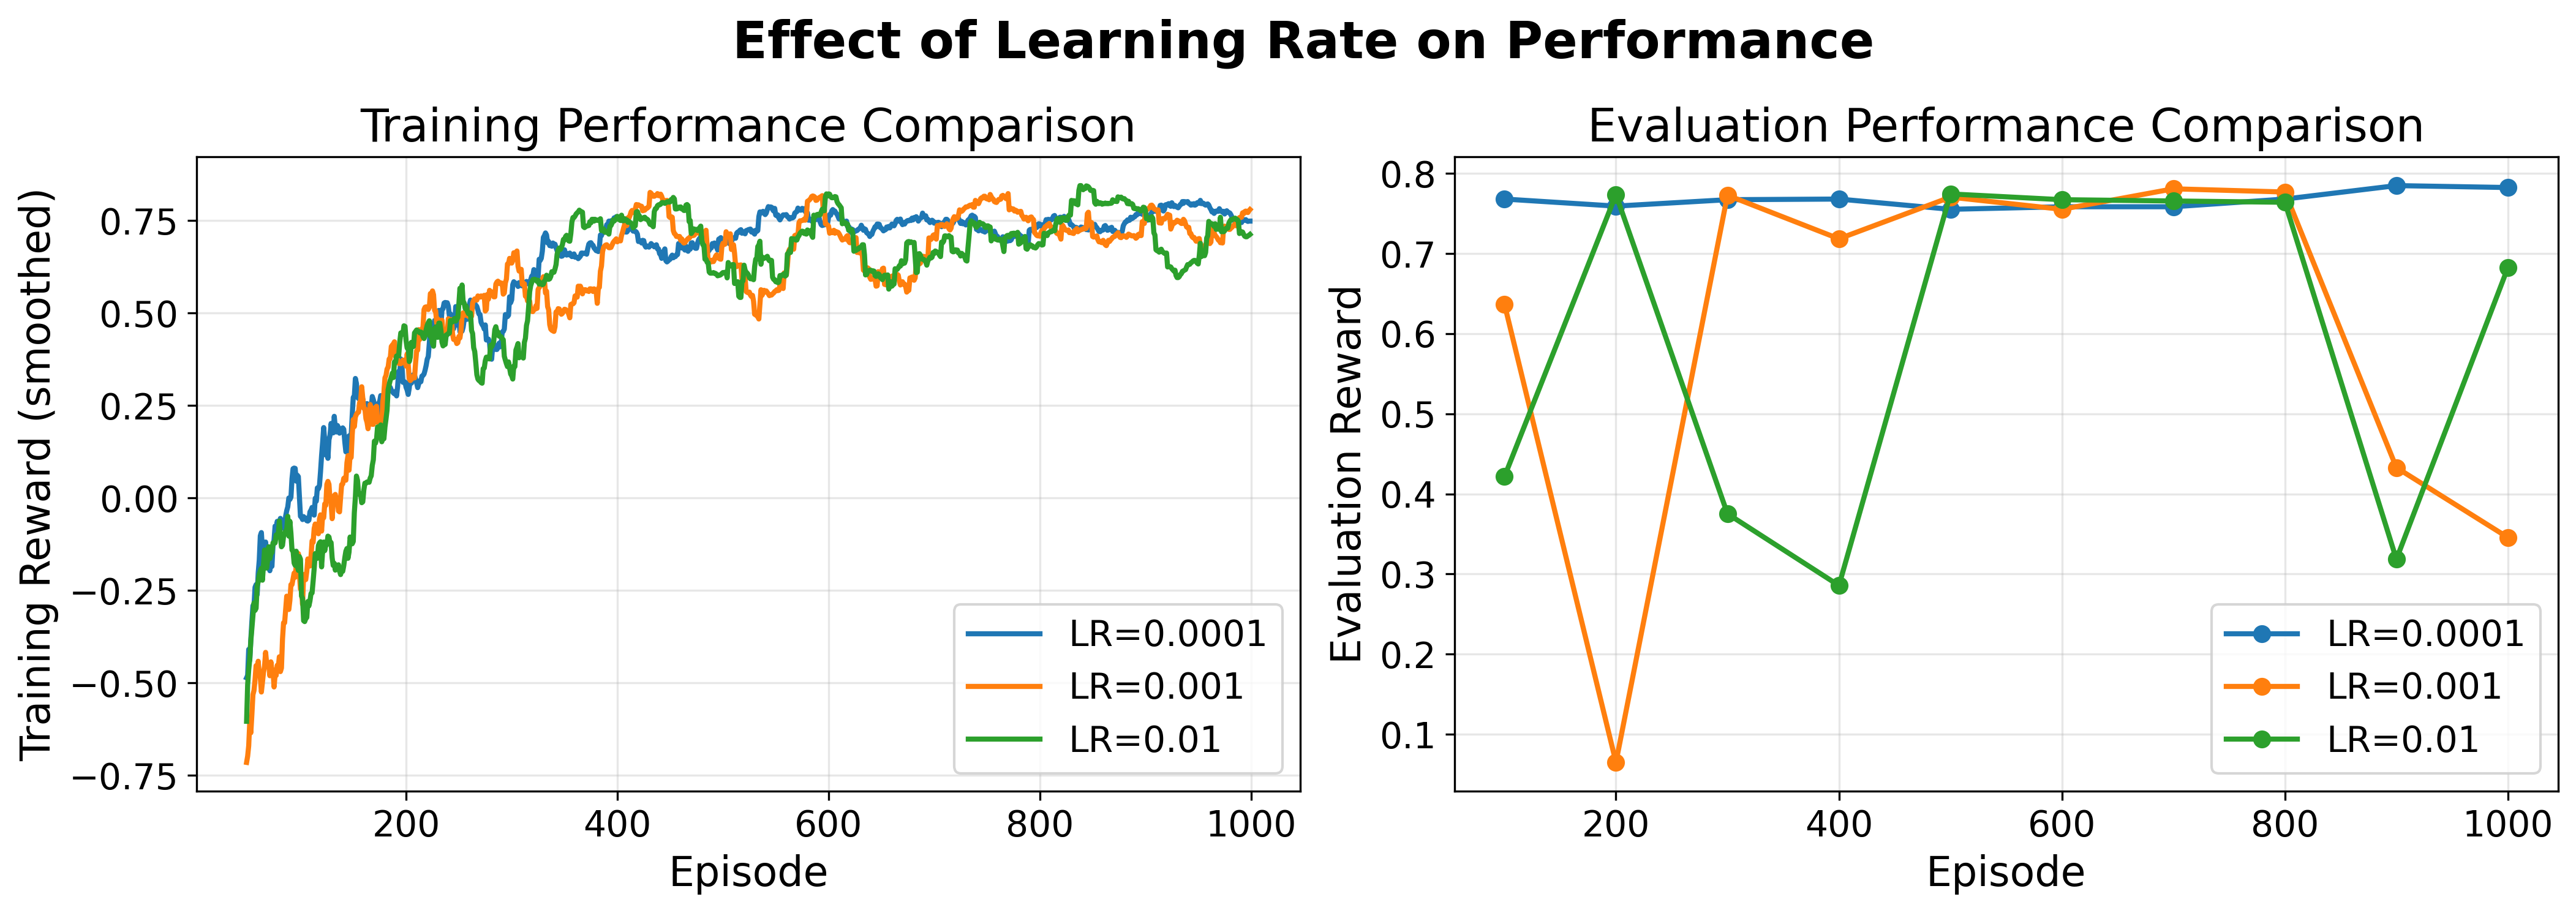
\includegraphics[width=\columnwidth]{images/experiment_learning_rate.png}}
\caption{Learning rate comparison across three values. The middle ground ($\alpha=0.001$, orange) converges fastest to the highest reward while maintaining stability. Too low is safe but slow; too high is fast but unstable.}
\label{fig:lr}
\end{figure}

Our chosen value of 0.001 (orange) hits the sweet spot: fast enough to converge in reasonable time, stable enough to maintain performance once learned. This reinforces conventional wisdom in deep learning about learning rates being critical yet problem-dependent.

\subsubsection{Network Architecture Exploration}

How much network capacity does a 12-state problem need? Figure \ref{fig:arch} provides surprising insights. A single hidden layer with 32 neurons (blue) proves insufficient, struggling to represent the optimal policy and plateauing around 0.68 reward.

\begin{figure}[htbp]
\centerline{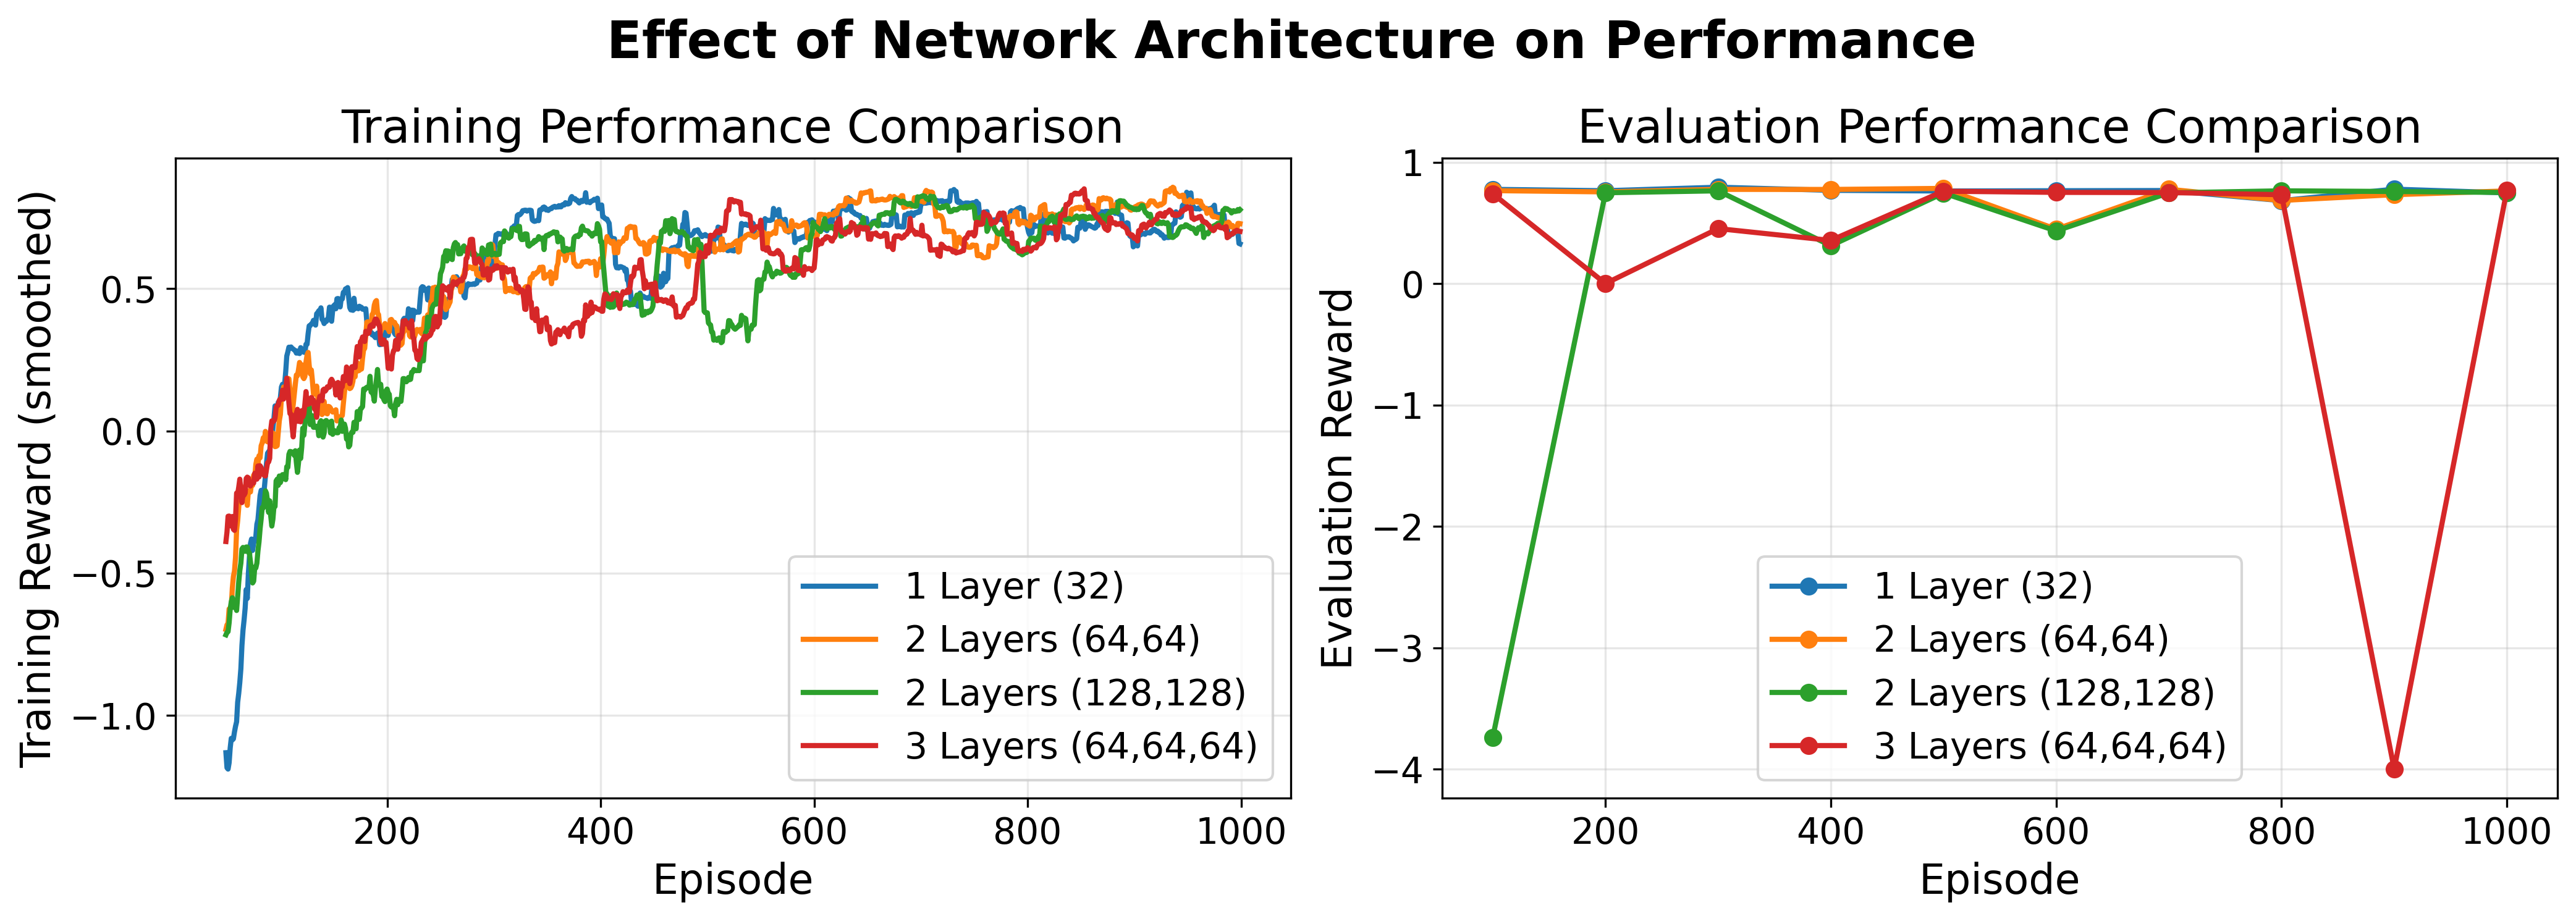
\includegraphics[width=\columnwidth]{images/experiment_architecture.png}}
\caption{Network architecture comparison from simple to complex. Two layers with 64 neurons each (orange) achieves best performance. More capacity doesn't help—the three-layer network (red) even shows instability with sudden drops.}
\label{fig:arch}
\end{figure}

Two layers with 64 neurons each (orange) work excellently, achieving our best 0.82 reward. Interestingly, adding more capacity—either more neurons per layer [128,128] (green) or more layers [64,64,64] (red)—doesn't improve results. The three-layer network actually shows instability, with evaluation performance occasionally dropping dramatically. This suggests that for small state spaces, compact networks may train more reliably than overparameterized ones.

\subsubsection{Balancing Exploration and Exploitation}

The epsilon decay rate determines how quickly we shift from exploration to exploitation. Figure \ref{fig:epsilon} demonstrates this tradeoff's importance. Fast decay (0.99, blue) commits to a greedy policy by episode 400 but achieves only 0.72 reward—the agent hasn't explored enough to find optimal paths.

\begin{figure}[htbp]
\centerline{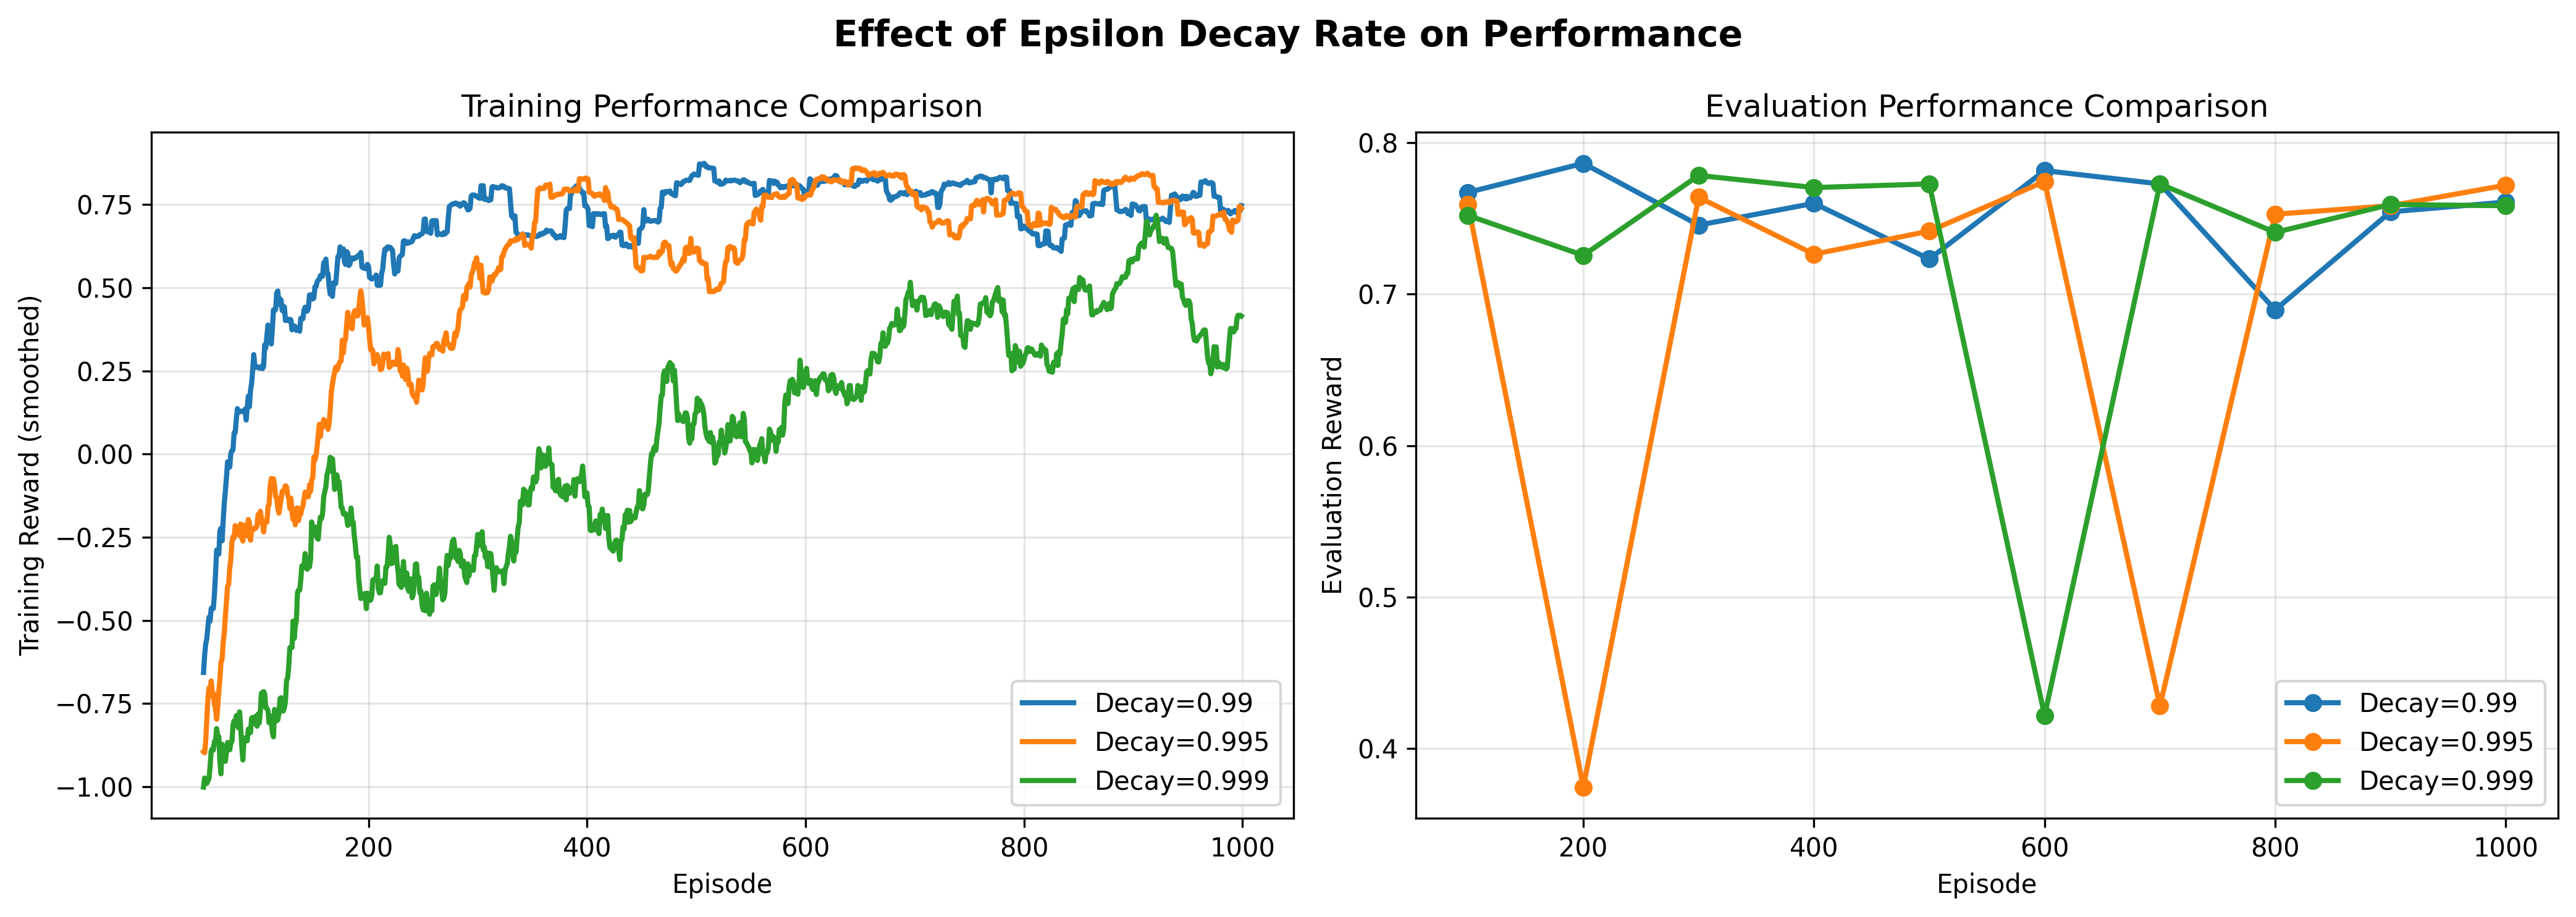
\includegraphics[width=\columnwidth]{images/experiment_epsilon.png}}
\caption{Epsilon decay rate comparison. Too fast (0.99, blue) leads to premature exploitation and suboptimal policies. Too slow (0.999, green) wastes episodes on excessive exploration. Our chosen rate (0.995, orange) balances these concerns effectively.}
\label{fig:epsilon}
\end{figure}

Slow decay (0.999, green) maintains substantial exploration even after 1,000 episodes, which seems wasteful once the agent has discovered good behaviors. Our middle-ground choice (0.995, orange) allows thorough early exploration while transitioning to exploitation around episode 900, yielding the best final performance.

\subsubsection{Batch Size Considerations}

Batch size affects both learning dynamics and computational efficiency. Figure \ref{fig:batchsize_plot} shows that small batches (16, blue) provide noisy gradient estimates, leading to faster but less stable updates. Large batches (128, red) smooth gradients but slow learning and increase computation time.

\begin{figure}[htbp]
\centerline{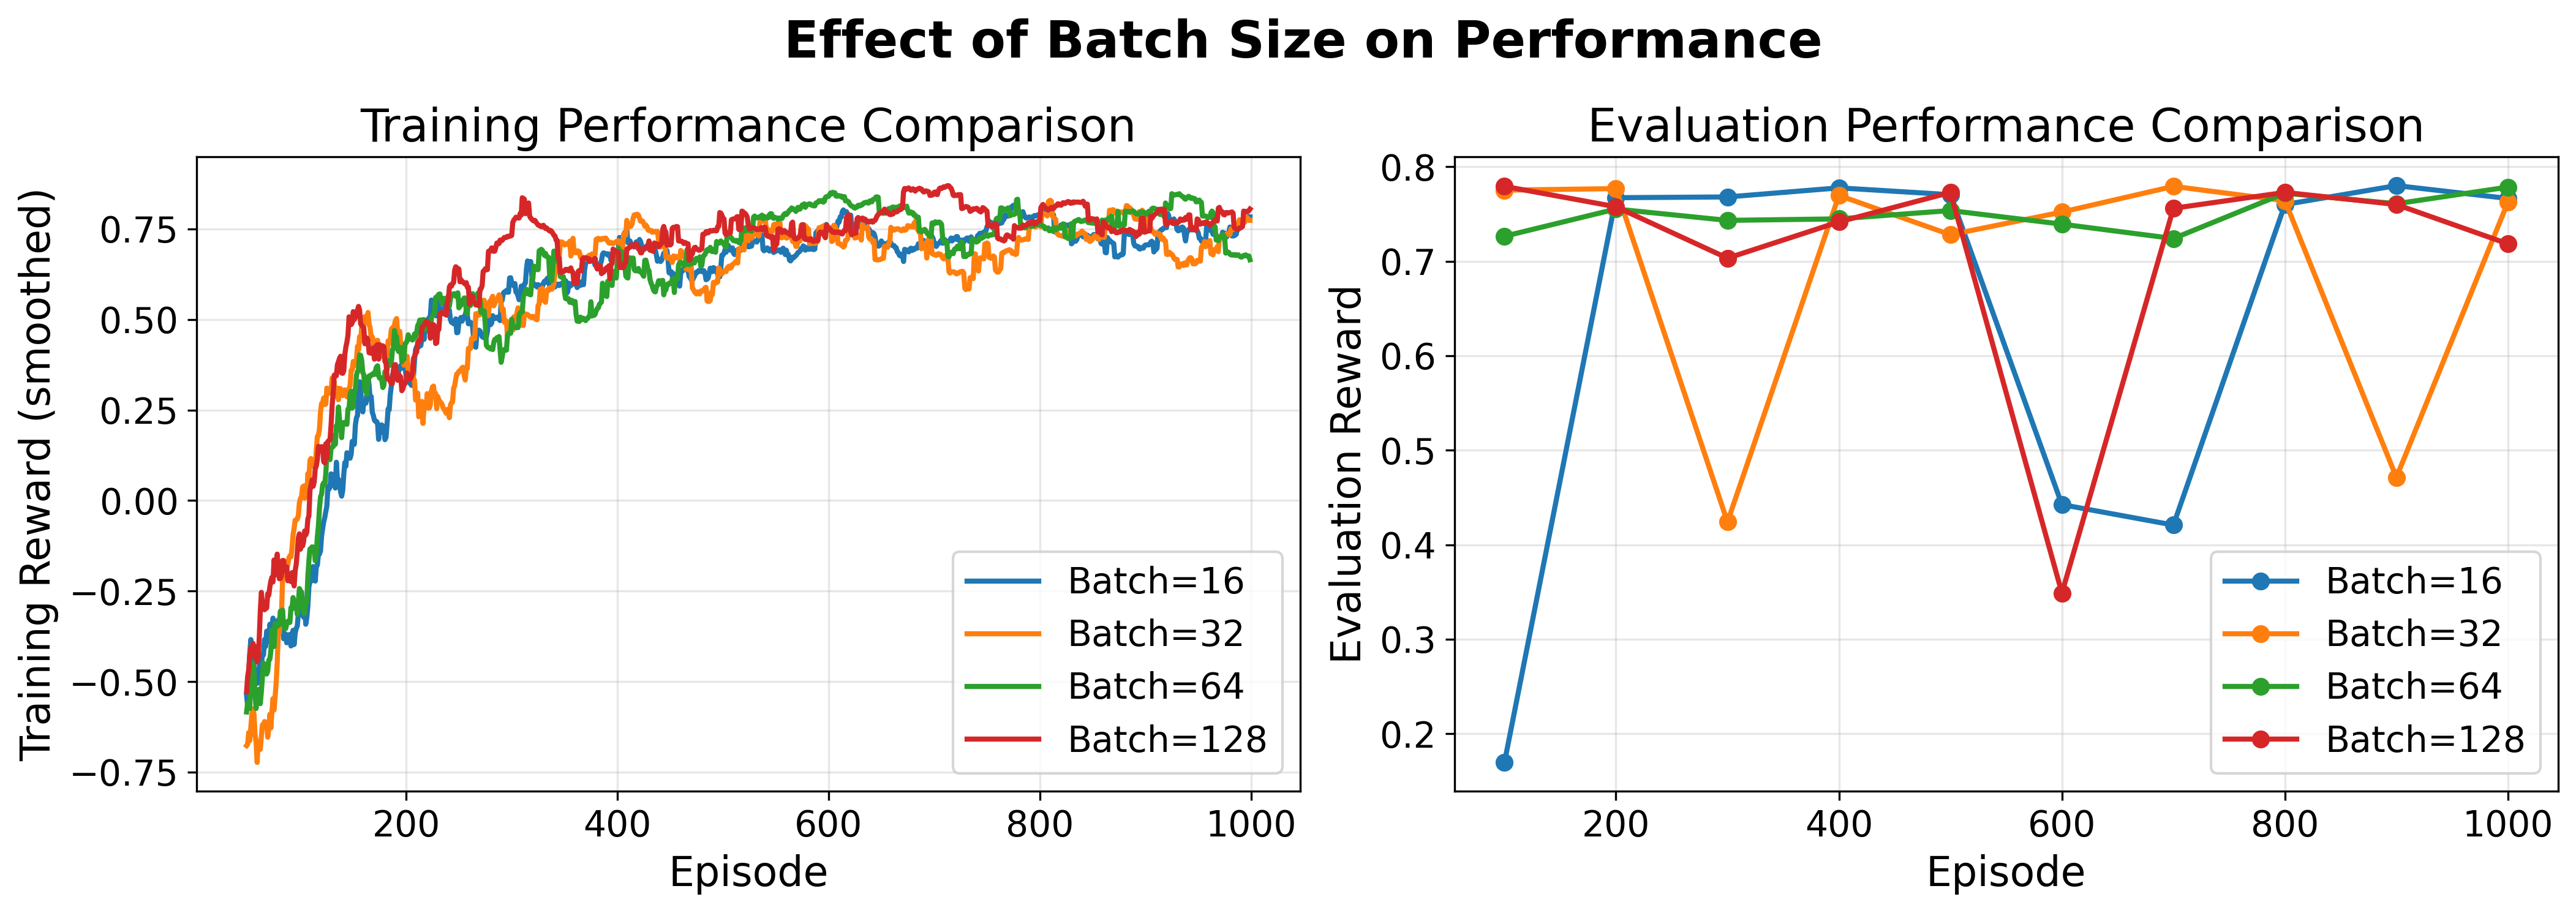
\includegraphics[width=\columnwidth]{images/experiment_batch_size.png}}
\caption{Batch size effects on learning. Small batches (16, blue) are fast but noisy. Large batches (128, red) are smooth but slow. Batch size 32 (orange) offers the best practical compromise.}
\label{fig:batchsize_plot}
\end{figure}

Our choice of 32 (orange) represents a practical compromise, achieving stable learning without excessive computational cost. This aligns with common practice in deep learning, where moderately-sized batches often work best.

\subsubsection{Planning Horizon Through Discounting}

The discount factor $\gamma$ controls how much the agent values future versus immediate rewards. Figure \ref{fig:gamma} shows that low values ($\gamma=0.9$, blue) create myopic policies focused on immediate costs, achieving only 0.73 reward. These agents undervalue the distant +1 goal relative to the -0.04 step costs.

\begin{figure}[htbp]
\centerline{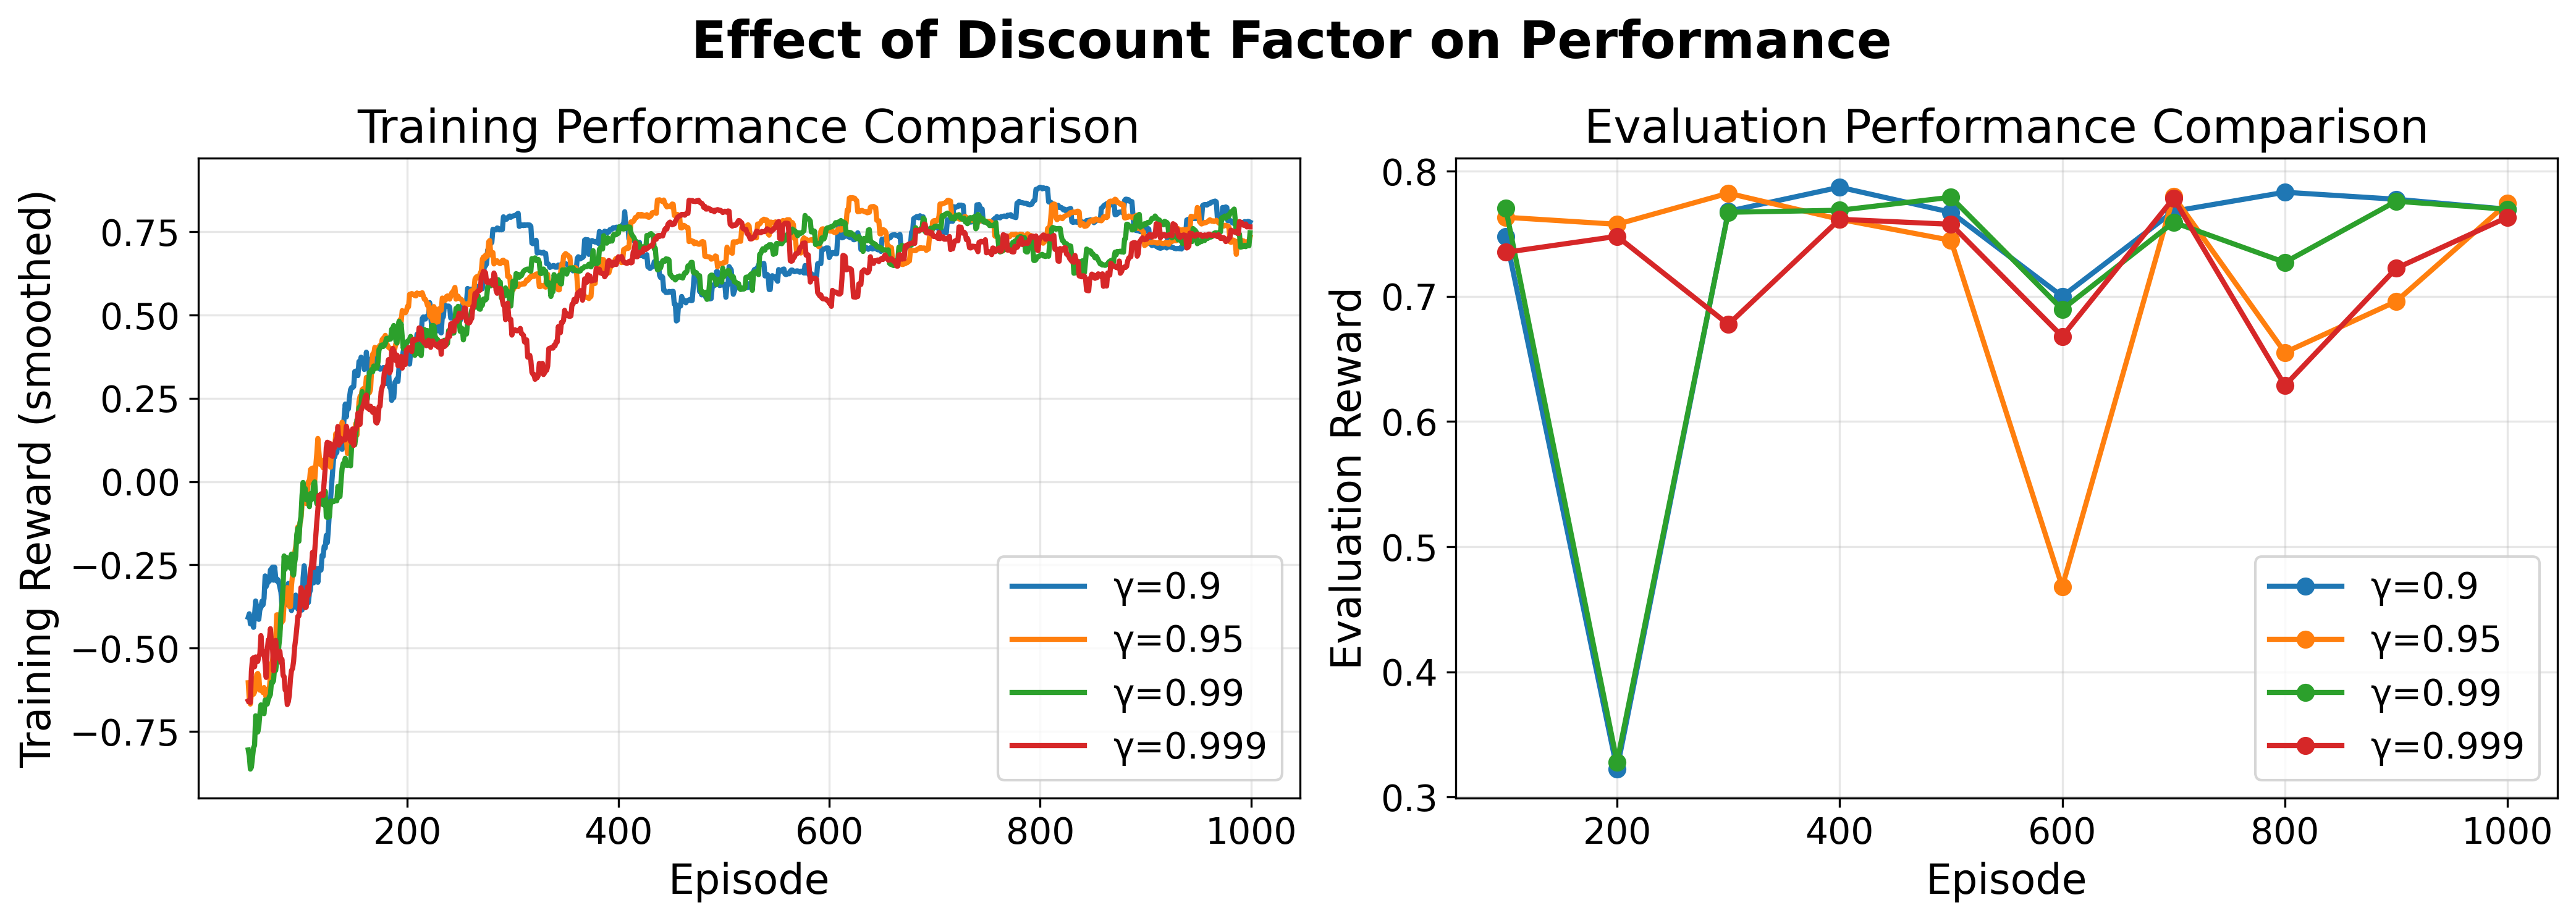
\includegraphics[width=\columnwidth]{images/experiment_gamma.png}}
\caption{Discount factor comparison showing planning horizon effects. Low gamma (0.9, blue) produces shortsighted policies. High gamma (0.99, green) appropriately values the long-term goal for this episodic task.}
\label{fig:gamma}
\end{figure}

Our chosen value of 0.99 (green) encourages long-term thinking appropriate for this task. Increasing further to 0.999 (red) provides no meaningful benefit—the episodes are short enough (typically 5-10 steps) that the difference between these high discount factors becomes negligible.

\subsection{Learned Policy Analysis}

What strategy did our agent ultimately learn? Analysis of the converged policy reveals it discovered the intuitive optimal path: move north twice to reach row 0, then move east three times to reach the goal. This 5-step path minimizes both step costs and trap risk.

Interestingly, the agent also learned appropriate caution. In state (0,2)—adjacent to both terminal states—the policy strongly prefers moving toward the goal rather than risking the trap, despite stochastic transitions occasionally causing unintended movements. This robustness to environmental noise was precisely our learning objective.

\subsection{Practical Insights}

Several implementation details proved more important than we initially expected. Gradient clipping (max norm 1.0) prevented occasional large updates when the agent stumbled into terminal states. Xavier initialization sped early learning substantially compared to random initialization. Experience replay's effectiveness surprised us—even with such a small state space, breaking temporal correlation reduced training variance significantly.

The computational efficiency of our approach is noteworthy. On a modern GPU, 2,000 training episodes complete in approximately 10 minutes. This rapid iteration enabled the extensive hyperparameter exploration reported here, illustrating how even with limited computational resources, systematic experimentation remains feasible for problems of this scale.

\section{Conclusion}

This work demonstrates that Deep Q-Networks can effectively solve stochastic gridworld navigation through careful algorithm design and hyperparameter tuning. Our implementation achieves near-optimal performance (0.82±0.05 reward, ~90\% success rate) by combining neural network function approximation with experience replay and target networks.

Our hyperparameter study yielded several practical insights: learning rate critically balances convergence speed and stability; network capacity should match problem complexity; exploration-exploitation balance requires careful tuning; moderate batch sizes work best; and discount factors should reflect task horizons. These findings may help practitioners applying DQN to similar problems.

While our small gridworld might seem toy-like, it captures essential challenges—stochastic dynamics, sparse rewards, navigation in continuous space—that appear in practical applications. The techniques we employed scale naturally to larger problems, with neural networks providing increasingly valuable function approximation as state spaces grow.

Future work could explore several interesting directions. Double DQN \cite{van2016deep} might reduce overestimation bias. Prioritized experience replay \cite{schaul2015prioritized} could improve sample efficiency. Dueling network architectures \cite{wang2016dueling} might better separate state value from action advantages. Extending to partially observable settings would add another layer of challenge.

The complete implementation, including all code, experiments, and results, is available at: \url{https://github.com/Jeevan-HM/RL-in-Robotics/tree/assignment_q_nn}.

\section*{Acknowledgment}

I thank my course instructor for the problem specification and helpful guidance throughout this project. I'm also grateful for the computational resources provided by Arizona State University that enabled the extensive experimentation reported here.

\begin{thebibliography}{00}
\bibitem{sutton2018reinforcement} R. S. Sutton and A. G. Barto, \textit{Reinforcement Learning: An Introduction}, 2nd ed. Cambridge, MA: MIT Press, 2018.

\bibitem{mnih2015human} V. Mnih et al., ``Human-level control through deep reinforcement learning,'' \textit{Nature}, vol. 518, no. 7540, pp. 529--533, 2015.

\bibitem{glorot2010understanding} X. Glorot and Y. Bengio, ``Understanding the difficulty of training deep feedforward neural networks,'' in \textit{Proc. 13th Int. Conf. Artificial Intelligence and Statistics}, 2010, pp. 249--256.

\bibitem{van2016deep} H. van Hasselt, A. Guez, and D. Silver, ``Deep reinforcement learning with double Q-learning,'' in \textit{Proc. AAAI Conf. Artificial Intelligence}, 2016, pp. 2094--2100.

\bibitem{schaul2015prioritized} T. Schaul et al., ``Prioritized experience replay,'' in \textit{Proc. Int. Conf. Learning Representations}, 2016.

\bibitem{wang2016dueling} Z. Wang et al., ``Dueling network architectures for deep reinforcement learning,'' in \textit{Proc. Int. Conf. Machine Learning}, 2016, pp. 1995--2003.

\bibitem{pytorch} A. Paszke et al., ``PyTorch: An imperative style, high-performance deep learning library,'' in \textit{Advances in Neural Information Processing Systems}, 2019, pp. 8024--8035.

\end{thebibliography}

\end{document}